\chapter{System Design}
\label{ch:system-design}

This chapter presents the design, implementation, and technical evaluation of a passwordless document encryption system. Section~\ref{sec:design-requirements} establishes the design requirements. Sections~\ref{sec:tech-selection} and~\ref{sec:architecture} describe the technology selection and system architecture. Section~\ref{sec:implementation} walks through the implementation, and Section~\ref{sec:eval-requirements} evaluates the system against the design requirements.

\section{Design Requirements}
\label{sec:design-requirements}

Based on the analysis of currently available solutions for document encryption and the limitations and gaps identified in Chapter~\ref{ch:evaluation}, and motivated by the repeated exploitation of systematic weaknesses in existing MFT platforms described in Section~\ref{sec:threat-analysis}, this section presents the design requirements of an ideal system outlined in research question R2: \emph{How can open-source protocols be used to design a document protection system that is passwordless, non-proprietary, and provides per-file encryption?} In this context, \emph{passwordless} has the meaning of no password or memory aspect is needed for the scheme to work, \emph{non-proprietary} has the meaning of being free, open-source and when files are shared, the receiver doesn't need custom software to view or interact with the file, and \emph{per-file encryption} has the meaning of individual document files are encrypted uniquely and not all accessible at once.

The threat model presented in Section~\ref{sec:threat-summary} identified four specific threats that the design must counter: (1)~bulk server-side file access, requiring granular per-document encryption without a single shared key; (2)~brute-force password cracking post-exfiltration, requiring passwordless key derivation; (3)~unauthorized redistribution of exfiltrated files, requiring recipient-bound encryption; and (4)~server compromise exposing keys, requiring non-custodial, client-side key derivation where the server never holds private keys. The evaluation framework presented in Chapter~\ref{ch:evaluation} produced 15 benefits across three categories---usability, security, and deployability---that an ideal document encryption system should satisfy (see Table~\ref{tab:evaluation-criteria}). These 15 benefits encompass the properties necessary to counter the threats identified in Section~\ref{sec:threat-summary} and serve as the formal design requirements for the system described in this chapter. One additional property, support for post-quantum cryptographic algorithms and cryptographic agility, is included as a design goal given the evolving threat landscape but was not part of the original evaluation framework. D4 (Mature) is acknowledged as unachievable for a prototype system and is discussed as a limitation in Chapter~\ref{ch:discussion}.

\section{Technology Selection}
\label{sec:tech-selection}

The passwordless document encryption system relies on three primary technologies: age encryption, specifically the typage TypeScript implementation, for file encryption; W3C's WebAuthn for the authentication ceremony; and FIDO2's CTAP for passkey or security key creation and communication. This section describes each technology and the rationale for its selection.

\subsection{age Encryption and typage}
\label{sec:age-typage}

Age is an open-source, modern file encryption tool and format. Initially developed as a Go library, the age specification has been implemented in several programming languages and supports plugins and integrations with several encryption management tools~\cite{age_repo}. Age encrypts arbitrary files for one or multiple recipients, where each recipient can independently decrypt the file to access the original plaintext. An age file is essentially a bundle made of two parts: a header and an encrypted payload. The header carries a 128-bit symmetric file key, generated from a cryptographically secure random source and unique to each file, encrypted (or ``wrapped'') independently for each designated recipient~\cite{stauble_age_thesis}. This wrapped file key is sent along with the encrypted payload so that it can be unwrapped by one or more of the corresponding identities.

Age was selected for this system for several reasons. First, it is open-source software licensed under BSD-3-Clause for free use, distribution, and modification~\cite{age_repo} satisfying the non-proprietary requirement (D5) and ensuring no licensing fee compromises negligible cost per user (D1). The age project is fairly mature (D4) with over 22{,}000 stars on GitHub at the time of writing and an active community of contributors~\cite{age_repo}. Second, age supports multi-recipient encryption natively: a file can be encrypted to multiple recipients, each of whom can decrypt independently using their own key material. This directly enables recipient-bound encryption (S4) and seamless sharing (U5). Third, age provides cryptographic agility through its support for multiple recipient types and its plugin architecture. As of version 1.3.0, age includes native support for hybrid post-quantum recipients using MLKEM768-X25519, providing resistance against future quantum computing attacks~\cite{age_spec}. Fourth, age's design keeps the encryption format simple and auditable compared to more complex formats such as PGP.

Typage is the official TypeScript implementation of age file encryption, available as an npm package or as a bundled JavaScript file~\cite{typage_repo}. Typage depends only on the noble cryptography libraries and uses the Web Crypto API when available. Typage was selected for the system implementation because TypeScript interfaces directly with the WebAuthn APIs available in the browser, and because a browser-based architecture satisfies several deployability requirements: users interact with a familiar web interface (U3) rather than downloading standalone software (D3, D6), no client-side software installation or updates are required, and the system can be updated centrally in a SaaS model.

\subsection{WebAuthn PRF Extension}
\label{sec:prf-tech-selection}

As discussed in Section~\ref{sec:webauthn-prf}, the WebAuthn PRF extension enables a passkey to serve not only as a login credential but also as a source for deriving symmetric encryption keys without passwords or server-stored secrets. In the designed system, the PRF extension is the critical bridge between FIDO2 authentication and age file encryption, enabling the system to derive encryption keys directly from a WebAuthn ceremony rather than from a user-supplied password.

Typage supports this model by interfacing with the WebAuthn API. When a user encrypts a file, typage triggers a WebAuthn ceremony in the browser. The browser prompts the user to select a passkey associated with the relying party ID (the website). During that WebAuthn ceremony, the PRF extension takes the authenticator's secret and the relying party ID and derives a deterministic symmetric key. That derived key is then used as the age file key to encrypt the file. To decrypt, the same process runs in reverse: the same passkey produces the same PRF output, yielding the same key, and the file decrypts. The identity string returned by the credential creation function can be provided at encryption or decryption time to ensure the user selects the correct passkey~\cite{typage_repo}.

This architecture delivers several of the design requirements identified in Section~\ref{sec:design-requirements}. The system is passwordless: the user never types or remembers a password but instead approves a biometric or passkey prompt (U1). It is non-custodial: the key is derived locally during the WebAuthn ceremony and no server sees it (S3). It is phishing-resistant: the derived key is scoped to the relying party ID, so a different domain produces a different key (S1). It supports both synced and hardware-bound authenticators: users can use synced passkeys through a passkey provider like iCloud Keychain, Google Password Manager, or 1Password for portability and recovery, or can choose hardware-bound keys such as a YubiKey for stronger security guarantees. This flexibility directly addresses the complementary strengths identified by Lyastani et al.\ and B\"uttner et al.\ as discussed in Sections~\ref{sec:fido2-evals} and~\ref{sec:eval-passwordless}: hardware-bound credentials provide strong security without a trusted third party while synced credentials provide portability and recovery (U4). By supporting both form factors, the system offers the strengths of each and enables each user to choose which mode is better for their specific use case.

\subsection{OpenTDF}
\label{sec:opentdf}

The system incorporates elements of the Open Trusted Data Format (OpenTDF) specification as scaffolding for future attribute-based access control (ABAC) capabilities. OpenTDF defines a structure consisting of a metadata manifest and an encrypted payload, where the manifest holds instructions for decryption and access control~\cite{opentdf_spec}. This architecture resembles the age header and encrypted payload model but expands it by including access control policies aligned with the NIST model for ABAC~\cite{nist_abac}.

The designed system's encrypted bundle format combines the age header with an OpenTDF-style manifest field, both preceding the encrypted data payload. The age header carries the wrapped file key for each recipient as described in Section~\ref{sec:age-typage}, while the manifest provides a structural placeholder for access control metadata such as recipient policies and expiration rules which would enable more advanced granular protection (S4). In the current implementation, the OpenTDF integration is limited to this structural scaffolding; a more complete ABAC implementation where the policy travels with the file is discussed as future work in Chapter~\ref{ch:discussion}.

\section{System Architecture}
\label{sec:architecture}

The system architecture is presented through four diagrams that progress from foundational to extended. The first presents the offline, client-only model: the basic building blocks of two users exchanging an encrypted file. The second shows the cloud/server-based model, which extends the offline architecture to include a server that hosts the encrypted bundle and enables updating contents, permissions, and sharing. The third and fourth diagrams depict two additional user actions within the cloud/server-based model: requesting access to a file (as recipient) and sharing access via a link (as sender).

Of these four, the cloud/server-based model was fully implemented and served as the basis for the user study described in Chapter~\ref{ch:user-study}. The offline model represents the foundational building blocks and is feasible but was not implemented as a standalone mode (see Appendix~\ref{ap:system-diagrams}). The request access and share access link flows are presented as theoretical extensions to illustrate how the architecture could support these interactions; structural scaffolding for them exists in the codebase (e.g., a share link button) but they were not fully implemented (see Appendix~\ref{ap:system-diagrams}). The user study focused on the core process of encrypting, decrypting, and sharing documents from the perspective of the sender rather than the full breadth of access management features and the receiving perspective. This was chosen in order to evaluate user acceptance and usability of the most fundamental interactions first.

The architecture diagrams build on the fundamentals of symmetric and asymmetric (public-private key) encryption. The following terms are used throughout:

\begin{description}
    \item[Alice:] The first user who has the file to encrypt and transmit.
    \item[Bob:] The second user who does not begin with the file but will receive or request access to it.
    \item[Private owner key:] The cryptographic key used to perform the encryption of the file, distinct from the private keys of other users who will access the file but did not perform the encryption.
    \item[Public key(s):] The cryptographic keys shared by Alice's associates, used to demonstrate their identity through the public-private key pair they hold.
    \item[Encrypted bundle:] The encrypted file containing the encryption informational header and the ciphertext. Called a bundle because the single file contains both the header metadata about the encryption and the actual encrypted data, drawing from the Open Trusted Data Format structure described in Section~\ref{sec:opentdf}.
\end{description}

\subsection{Offline/Client-Only Model}
\label{sec:offline-model}

The simplest expression of the architecture is the offline, client-only model (see Appendix~\ref{ap:system-diagrams}) in which two users exchange an encrypted file with no server involved. While this model primarily serves as the foundation for the cloud/server-based implementation, it has standalone applications in airgapped or self-hosted environments where system constraints may require deploying passwordless document encryption independent of any server or cloud access. This architecture also lends itself to containerization or microservice deployment. In the offline model, Alice creates a private owner key via WebAuthn PRF, specifies which public keys are valid recipients, bundles the encrypted file with the owner key reference and approved public key list, and transmits the bundle to Bob through any file transfer mechanism. Bob then verifies his identity by demonstrating he holds a private key matching one of the approved public keys, and decryption proceeds. The primary limitation is that once the bundle is sent, the owner cannot update permissions: the approved keys at the time of encryption are fixed.

\subsection{Cloud/Server-Based Model}
\label{sec:cloud-model}

The cloud/server-based model (Figure~\ref{fig:cloud-arch}) extends the offline architecture by introducing a server that hosts the latest encrypted bundle, enabling the owner to update permissions and file contents without redistributing the bundle.

\begin{figure}[htbp]
    \centering
    
\includegraphics[width=5.5in]{cloud-server-architecture}
    \caption[Cloud/server-based architecture.]{Cloud/server-based architecture. Alice generates the private owner key and uploads the encrypted bundle to the server, then can update permissions or contents at any time. Bob downloads the bundle, pulls the latest approved public key list, and verifies his identity to decrypt.}
    \label{fig:cloud-arch}
\end{figure}

The flow begins with Alice setting the private owner key and specifying which public keys have access to the file (step~1). The private owner key is generated through WebAuthn PRF via a FIDO2 passkey or other authenticator, which could be managed through a password manager, identity provider, or hardware token such as a YubiKey. By specifying who has access, Alice determines which public keys will be valid to decrypt the file. In step~2, Alice verifies her identity to demonstrate ownership of the private owner key. This may coincide with key creation---for example, a new passkey is created to serve as the owner key, or a YubiKey is tapped---or it may involve presenting an existing credential. In step~3, the encrypted bundle is uploaded to the server. Critically, the server only ever holds already-encrypted ciphertext and cannot decrypt the document because private keys remain at the client level and are not transmitted to or accessible by the server.

Step~4 introduces the key advantage of the server-based model over the offline architecture: Alice can update the approved public key list, remove the file, re-encrypt with a new owner key, or change other permissions at any time by repeating the process of steps~1--3 and uploading the updated bundle. In step~5, Bob downloads the encrypted bundle from the server. In step~6, Bob pulls the latest approved public key list. In step~7, Bob verifies his identity by demonstrating he holds a valid private key matching an approved public key. In step~8, decryption of the bundle proceeds if Bob's key pair matches an entry in the current approved public key list.

This model retains the core benefits of the offline architecture---no passwords, per-file encryption, recipient verification using the recipient's preferred authenticator---while adding the ability for the owner to modify permissions after sharing. The server hosts encrypted data and public key lists but has no ability to decrypt documents, preserving the non-custodial property. Even if the server is compromised, the attacker obtains only ciphertext and public keys, not the private keys needed for decryption.

\subsection{Request Access and Share Access Link Flows}
\label{sec:request-share-flows}

Two additional flows extend the cloud/server-based model to support common document sharing interactions: requesting access as a recipient and sharing access via a link as a sender. These flows are presented as architectural extensions in Appendix~\ref{ap:system-diagrams}.

The request access flow addresses the scenario where Bob wants to access a file Alice has already uploaded. Bob navigates to the server, requests access to a specific file, and provides his public key. The server forwards the request to Alice, who reviews and approves or denies it after verifying her identity as the owner. If granted, the server updates the approved key list and Bob can proceed to download and decrypt the file.

The share access link flow addresses the scenario where Alice proactively shares a file with Bob via a copied link, an interaction pattern familiar from cloud file sharing systems such as Dropbox, Google Drive, SharePoint, and Box. Alice generates a share link which is sent to Bob by email or another communication channel. When Bob opens the link, the server prompts him to provide a public key to associate with his identity, after which Alice can approve the association and Bob gains access.

\section{System Implementation Walkthrough}
\label{sec:implementation}

The system is implemented as a Next.js web application using React 19 and TypeScript, with age encryption provided by the typage library, credential storage in IndexedDB, and an optional Supabase backend for link sharing. The complete source code is available as an open-source repository~\cite{docprotect_repo}. This section walks through the implementation organized by user-facing workflow steps, corresponding to the guided workflow presented in the application interface.

\paragraph{File Upload.} The application presents a single interface for both encryption and decryption (Figure~\ref{fig:ui-upload}). The user uploads any file to encrypt it, or uploads a \texttt{.rico} file to decrypt it. The system detects the file type automatically and adjusts the workflow accordingly: encryption proceeds through a five-step flow (Upload, Identity, Recipients, Share, Done) while decryption uses a shortened three-step flow (Upload, Identity, Done).

\begin{figure}[htbp]
    \centering
    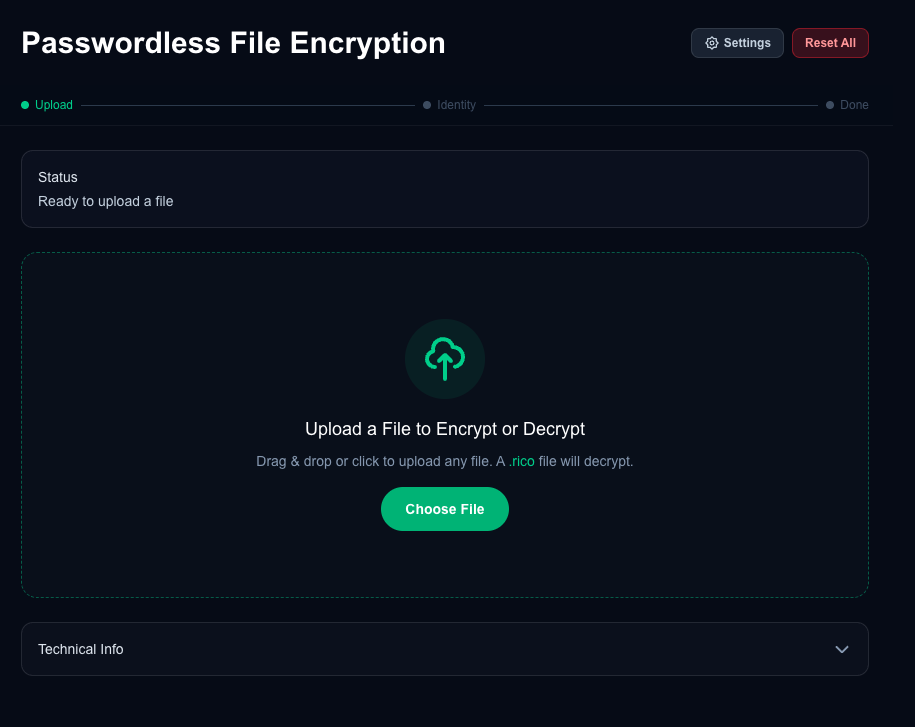
\includegraphics[width=5in]{figures/ui-upload.png}
    \caption{File upload interface of the DocProtect application.}
    \label{fig:ui-upload}
\end{figure}

\paragraph{Identity Verification (Encryption).} For encryption, the user verifies their identity by creating or selecting a passkey credential (Figure~\ref{fig:ui-identity}). The primary path presents a ``New Passkey'' option where the user sets a name for the credential (defaulted to the uploaded file's filename) and clicks ``Create \& Encrypt,'' which triggers a WebAuthn ceremony in the browser to create a credential (passkey or security key). Upon completion a second WebAuthn ceremony is immediately begun which uses the newly created credential to encrypt the file. The credential creation prompt comes from the user's default platform or third-party passkey provider (Figure~\ref{fig:ui-save-passkey}). The credential creation flow, including PRF detection and fallback handling, is detailed in the sequence diagram in Appendix~\ref{ap:system-diagrams}.

\begin{figure}[htbp]
    \centering
    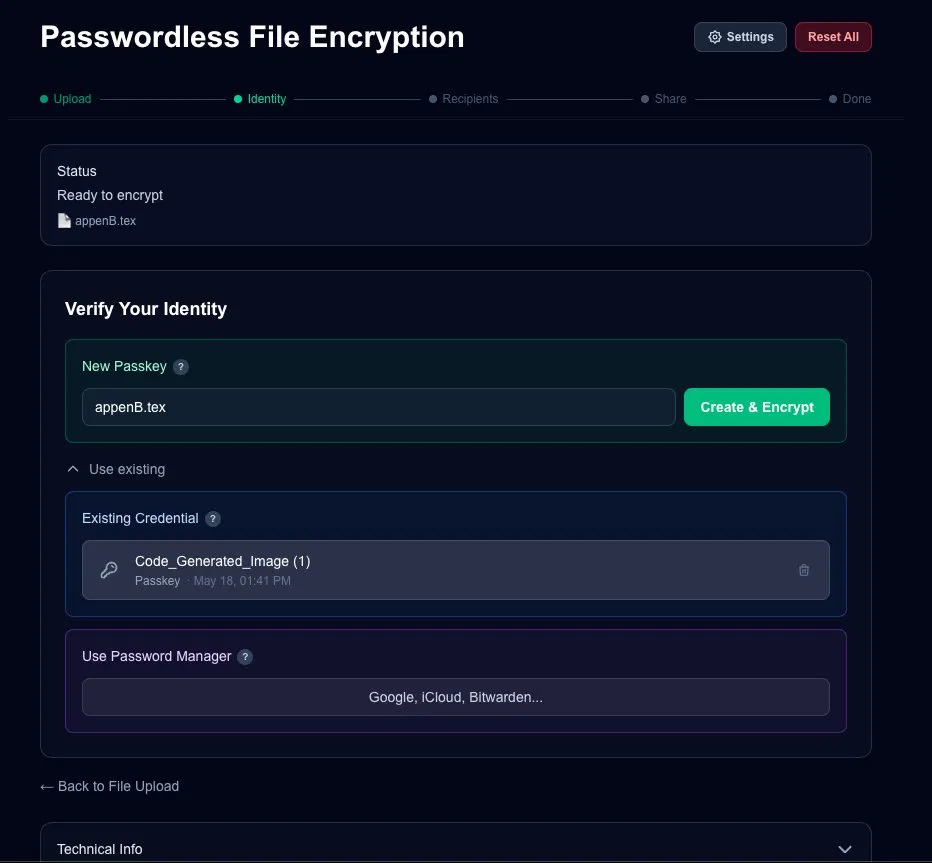
\includegraphics[width=5in]{figures/ui-identity.png}
    \caption{Identity verification step with the New Passkey option and Create \& Encrypt action.}
    \label{fig:ui-identity}
\end{figure}

\begin{figure}[htbp]
    \centering
    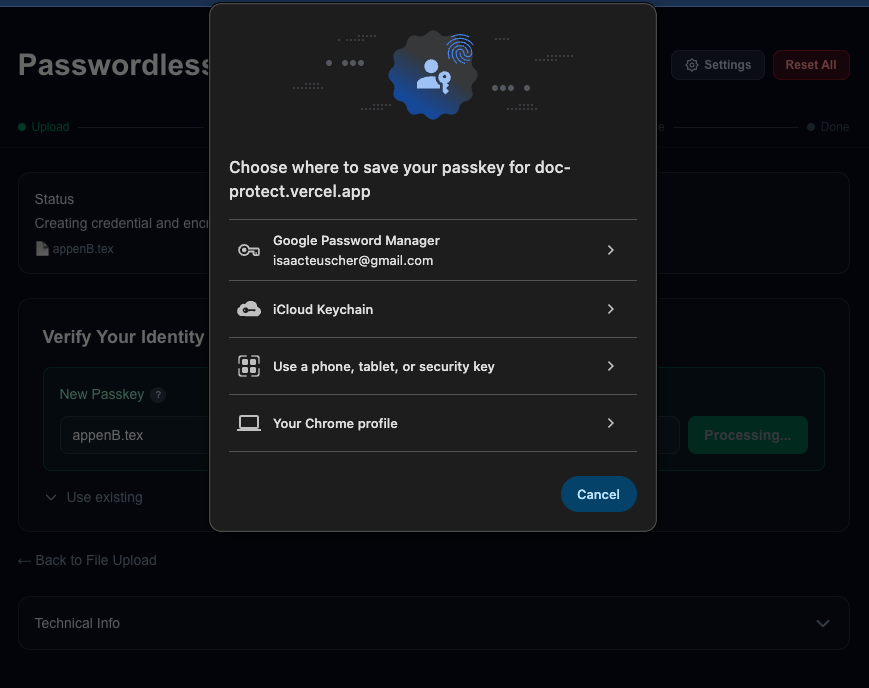
\includegraphics[width=5in]{figures/ui-save-passkey.png}
    \caption{Save-a-passkey prompts presented by the user's passkey provider during credential creation.}
    \label{fig:ui-save-passkey}
\end{figure}

An expandable ``Use existing'' section (Figure~\ref{fig:ui-use-existing}) provides two additional paths: selecting a previously created credential stored in IndexedDB, or using a passkey from an external password manager such as iCloud Keychain, Google Password Manager, or Bitwarden. Each stored credential displays its name and creation date, and can be deleted from IndexedDB.

\begin{figure}[htbp]
    \centering
    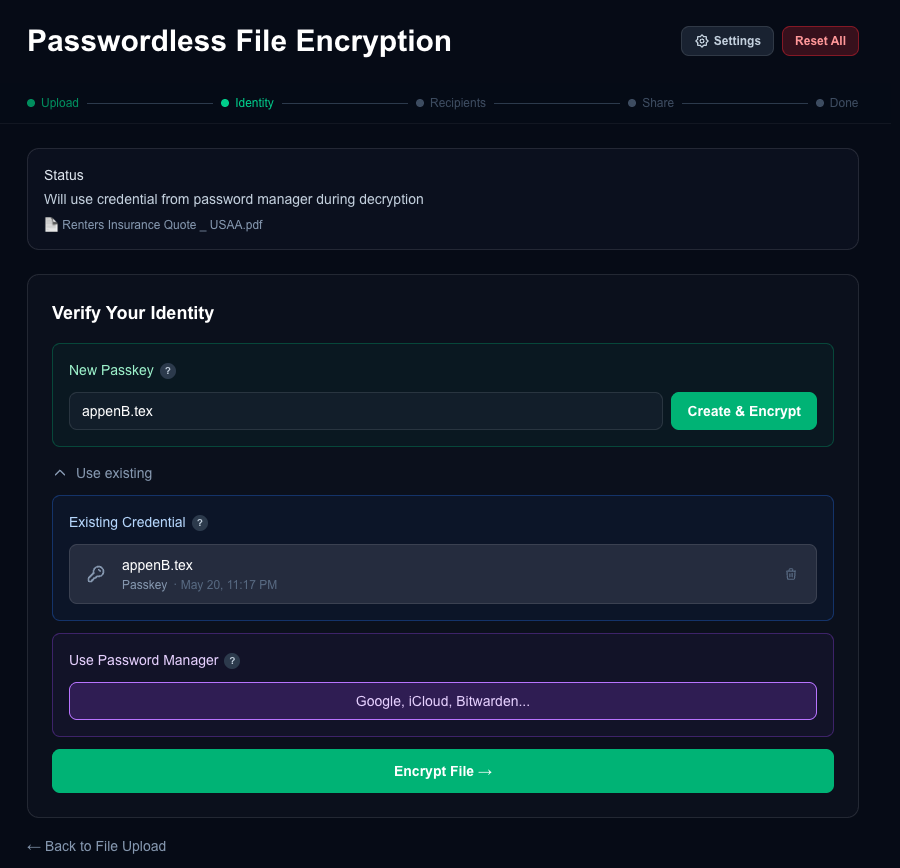
\includegraphics[width=5in]{figures/ui-use-existing.png}
    \caption{The ``Use existing'' panel for selecting a previously created or third-party credential.}
    \label{fig:ui-use-existing}
\end{figure}

\paragraph{Recipients.} After encryption, the user can optionally add recipients by email address (Figure~\ref{fig:ui-recipients}). Recipients can be added individually or as a comma-separated list. This step can also be skipped entirely for single-user encryption.

\begin{figure}[htbp]
    \centering
    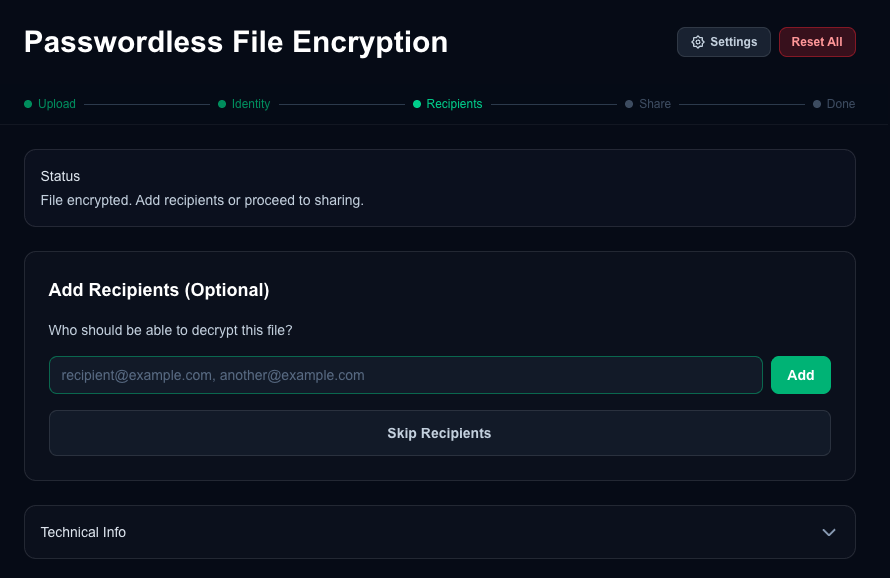
\includegraphics[width=5in]{figures/ui-recipients.png}
    \caption{Add-recipients step of the encryption workflow.}
    \label{fig:ui-recipients}
\end{figure}

\paragraph{Sharing.} The sharing step (Figure~\ref{fig:ui-share}) presents three options for distributing the encrypted file: downloading the bundle directly for manual sharing via email or messaging, uploading to cloud storage (Google Drive), or generating a shareable link via the Supabase backend. The download option produces a \texttt{.rico} file, which is a ZIP archive containing a \texttt{manifest.json} (metadata, policy, and recipient list) and a \texttt{0.payload} file (the age-encrypted data). The cloud storage and shareable link options create realistic-looking links but do not actually integrate with those file storage services to upload the bundle as the focus for this system was to develop a proof-of-concept that is realistic enough for user acceptance and usability testing of the core steps.

\begin{figure}[htbp]
    \centering
    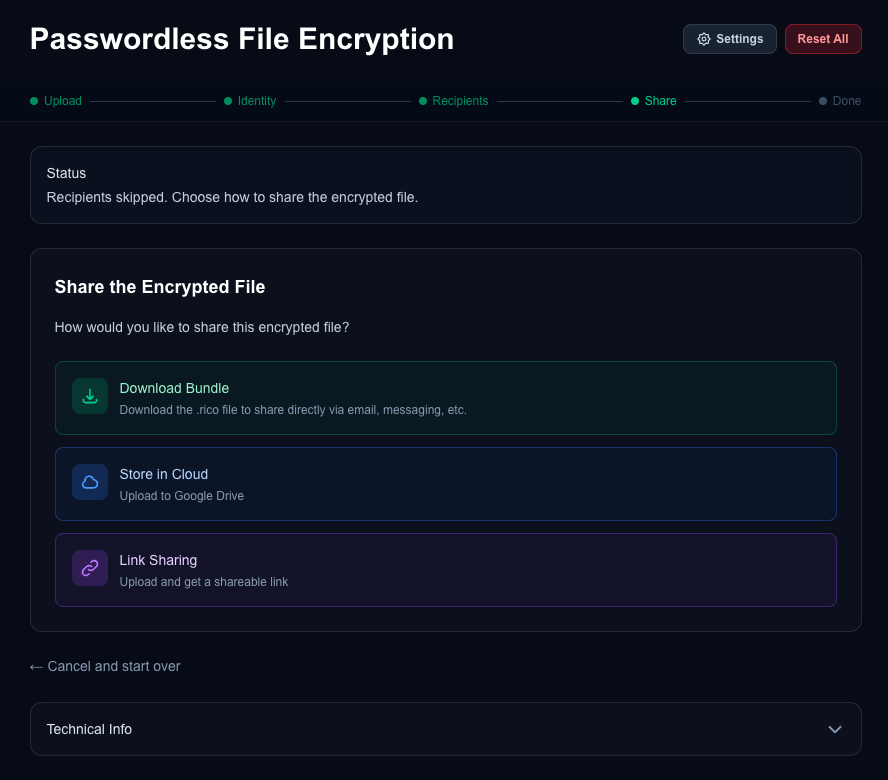
\includegraphics[width=5in]{figures/ui-share.png}
    \caption{Share options presented after encryption.}
    \label{fig:ui-share}
\end{figure}

\paragraph{Decryption.} When a \texttt{.rico} file is uploaded, the interface presents the decryption path (Figure~\ref{fig:ui-decrypt}). The user selects a stored credential or uses their password manager's passkey picker, then clicks ``Decrypt File.'' The system parses the bundle, extracts the manifest and encrypted payload, triggers a WebAuthn ceremony to derive the decryption key via PRF, and presents the decrypted file for download.

\begin{figure}[htbp]
    \centering
    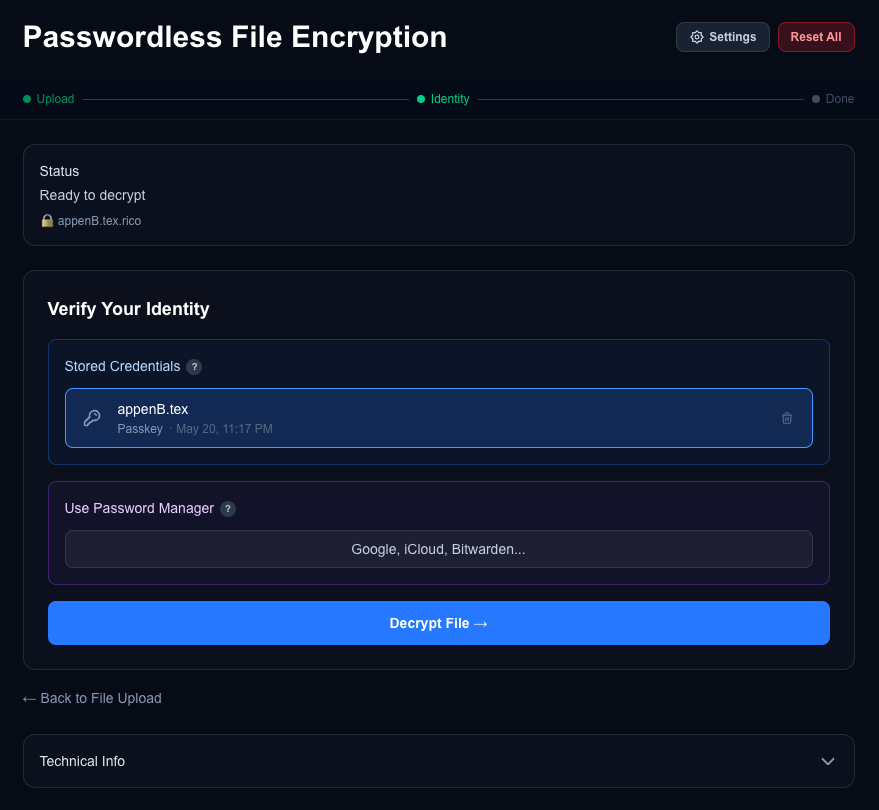
\includegraphics[width=5in]{figures/ui-decrypt.png}
    \caption{Decryption-side identity step with Decrypt File action.}
    \label{fig:ui-decrypt}
\end{figure}

\paragraph{Settings.} A settings panel (Figure~\ref{fig:ui-settings}) allows the user to select between three encryption algorithms: WebAuthn Passkey (PRF) as the default, Post-Quantum Hybrid (ML-KEM-768 + X25519), or Classic (X25519). This panel is collapsed by default.

\begin{figure}[htbp]
    \centering
    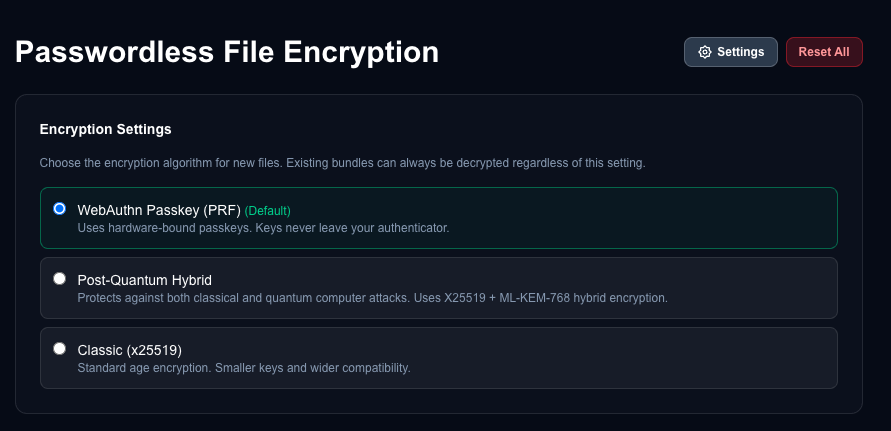
\includegraphics[width=5in]{figures/ui-settings.png}
    \caption{Settings panel with encryption algorithm selection.}
    \label{fig:ui-settings}
\end{figure}

\paragraph{Technical Information.} An expandable ``Technical Info'' panel (Figure~\ref{fig:ui-techinfo}) displays the current encryption algorithm setting, PRF support status for the platform, stored credentials with their type and PRF capability, and the current workflow state. This panel was included for transparency during the user study and for debugging during development.

\begin{figure}[htbp]
    \centering
    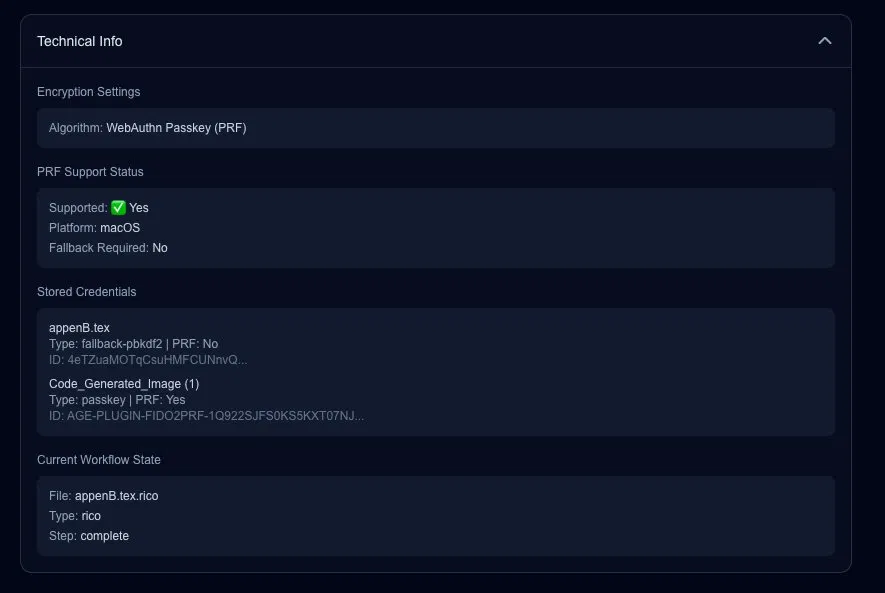
\includegraphics[width=5in]{figures/ui-techinfo.png}
    \caption{Technical Info panel for transparency and debugging.}
    \label{fig:ui-techinfo}
\end{figure}

\paragraph{Bundle Format.} The \texttt{.rico} bundle format is a ZIP archive containing two files: \texttt{manifest.json}, which stores file metadata, encryption algorithm, recipient list, and an OpenTDF-inspired policy object with ABAC scaffolding (see Section~\ref{sec:opentdf}); and \texttt{0.payload}, which contains the age-encrypted binary data. The manifest tracks the encryption algorithm used (\texttt{age}, \texttt{age-pq}, \texttt{age-x25519}, or \texttt{age-fallback}), enabling the system to select the correct decryption path automatically.

\paragraph{Technology Stack.} The implementation uses Next.js 16 as the application framework, the \texttt{age-encryption} npm package (typage) for all encryption operations, IndexedDB via localForage for local credential storage, JSZip for bundle creation and parsing, and Playwright for end-to-end testing. The application requires a modern browser with WebAuthn support. PRF is supported on macOS, iOS, Android, and Chrome OS platform authenticators, as well as YubiKey 5+ hardware tokens; Windows Hello added hmac-secret support in February 2026. A PBKDF2 fallback mode is provided for platforms without PRF support. The code was developed with assistance from Claude Code (Opus 4.6 AI model).

\section{Evaluation Against Requirements}
\label{sec:eval-requirements}

This section evaluates the implemented system against the 15 design requirements derived from the Chapter~\ref{ch:evaluation} evaluation framework. Table~\ref{tab:uds-evaluation} summarizes the evaluation, rating each benefit as fully satisfied, partially satisfied, or not satisfied, with justification.

\begin{table}[p]
    \centering
    \renewcommand{\arraystretch}{1.1} 
    \caption{Evaluation of Implemented System Against Design Requirements}
    \label{tab:uds-evaluation}
    \footnotesize
    \setlength{\tabcolsep}{3pt}
    \begin{adjustbox}{max width=\linewidth,center}
    \begin{tabularx}{\linewidth}{
        >{\bfseries\centering\arraybackslash}m{0.55cm} % ID Column
        >{\raggedright\arraybackslash}m{2.35cm}        % Benefit Column
        >{\raggedright\arraybackslash}m{1.85cm}        % Rating Column
        >{\raggedright\arraybackslash}X               % Justification Column
    }
        \toprule
        & \textbf{Benefit} & \textbf{Rating} & \textbf{Justification} \\
        \midrule
        
        % ==========================================
        % --- USABILITY ---
        % ==========================================
        U1 & Memorywise-Effortless & \CIRCLE\ Full & Users authenticate via passkey or security key (biometric or hardware tap). No passwords or secrets to remember. \\
        \arrayrulecolor{gray!40}\midrule\arrayrulecolor{black}
        
        U2 & Scalable-for-Users & \CIRCLE\ Full & Users' cognitive load does not increase with additional documents as individual secrets do not need to be remembered. \\
        \arrayrulecolor{gray!40}\midrule\arrayrulecolor{black}
        
        U3 & Easy-to-Learn & \CIRCLE\ Full & The guided step-by-step workflow mirrors familiar web interactions. Evaluated empirically in Chapter 6. \\
        \arrayrulecolor{gray!40}\midrule\arrayrulecolor{black}
        
        U4 & Easy-Recovery-from-Loss & \LEFTcircle\ Partial & Synced passkeys (e.g. iCloud, Google, 1Password) provide recovery through cloud backup. Hardware-bound credentials have no recovery path. Supporting both authenticator types gives users a choice based on their risk tolerance. \\
        \arrayrulecolor{gray!40}\midrule\arrayrulecolor{black}
        
        U5 & Seamless-Sharing & \LEFTcircle\ Partial & Direct download is implemented. Link sharing and the full recipient-initiated access request flow is scaffolded but not fully implemented. \\
        
        \midrule % <--- DARK SOLID LINE SEPARATING SECTIONS
        
        % ==========================================
        % --- DEPLOYABILITY ---
        % ==========================================
        D1 & Negligible-Cost-per-User & \CIRCLE\ Full & All components are open-source and free. No per-user licensing fees. \\
        \arrayrulecolor{gray!40}\midrule\arrayrulecolor{black}
        
        D2 & Negligible-IT-Support-Cost & \CIRCLE\ Full & Browser-based SaaS model requires no client installation, updates, or IT provisioning. \\
        \arrayrulecolor{gray!40}\midrule\arrayrulecolor{black}
        
        D3 & Compatible & \LEFTcircle\ Partial & Runs in any modern browser (Chrome 108+, Edge 108+, Safari 16.4+). PRF support depends on both the platform authenticator and operating system; Windows Hello added support in February 2026 and a PBKDF2 fallback is provided for unsupported platforms. \\
        \arrayrulecolor{gray!40}\midrule\arrayrulecolor{black}
        
        D4 & Mature & \Circle\ Not satisfied & The current system is a research prototype (v0.1). Maturity can only come as real-world deployment scale over time. Acknowledged as a limitation. \\
        \arrayrulecolor{gray!40}\midrule\arrayrulecolor{black}
        
        D5 & Non-Proprietary & \CIRCLE\ Full & \texttt{age} is BSD-3-Clause licensed. WebAuthn and FIDO2 are open W3C/FIDO Alliance standards. The codebase is open-source. \\
        \arrayrulecolor{gray!40}\midrule\arrayrulecolor{black}
        
        D6 & Guest-Friendly & \LEFTcircle\ Partial & Recipients can decrypt via their own passkey without provisioned accounts. The share link flow enabling access without prior credentials is scaffolded but not fully implemented. \\
        
        \midrule % <--- DARK SOLID LINE SEPARATING SECTIONS
        
        % ==========================================
        % --- SECURITY ---
        % ==========================================
        S1 & Resilient-to-Observation & \CIRCLE\ Full & No passwords to observe. The PRF-derived key exists only during the WebAuthn ceremony and is not displayed or typed. Phishing resistant through relying party bound credentials. \\
        \arrayrulecolor{gray!40}\midrule\arrayrulecolor{black}
        
        S2 & Resilient-to-Guessing & \CIRCLE\ Full & The encryption key is derived from the authenticator's internal secret via PRF, not from a user-chosen password. Offline brute-force and dictionary attacks are not feasible. \\
        \arrayrulecolor{gray!40}\midrule\arrayrulecolor{black}
        
        S3 & Resilient-to-Third-Party-Leak & \CIRCLE\ Full & Encryption keys are derived client-side and never leave the browser. The server only sees already-encrypted ciphertext. Server compromise yields no plaintext or key material. \\
        \arrayrulecolor{gray!40}\midrule\arrayrulecolor{black}
        
        S4 & Granular-Protection & \CIRCLE\ Full & Each document is encrypted with a unique file key. Compromise of one document does not grant access to others. \\
        
        \bottomrule
    \end{tabularx}
    \end{adjustbox}
\end{table}


The system in its current state fully satisfies 10 of the 15 benefits, partially satisfies 4, and does not satisfy 1 (D4-Mature). The four partial ratings reflect current state constraints rather than architectural limitations. Two partial ratings (U5-Seamless-Sharing and D6-Guest-Friendly) come from the proof-of-concept nature of the research reflecting the scoping decision to prioritize the core encryption workflow over the full access management feature set. These benefits could be fully satisfied with additional development. D3-Compatible reflects the current state of PRF platform support which is maturing rapidly. U4-Easy-Recovery-from-Loss depends on the user's choice of authenticator type and is rated as partial since it maintains the tradeoff decision between device-bound and synced passkeys.

\paragraph{Addressing the FIDO2 Gaps.} As discussed in Sections~\ref{sec:fido2-evals} and~\ref{sec:eval-passwordless}, Lyastani et al.\ identified four remaining gaps when applying FIDO2 hardware tokens to the Bonneau framework: Nothing-to-Carry, Easy-Recovery-from-Loss, Server-Compatible, and Resilience-to-Theft. B\"uttner et al.\ found that synced passkeys address portability and recovery but introduce third-party trust in the passkey provider. The designed system addresses these gaps by supporting both authenticator types. Synced passkeys provide Nothing-to-Carry (the credential is available on any device with the passkey provider), Easy-Recovery-from-Loss (backup and restore through the provider), and broader compatibility. Hardware-bound credentials provide no trusted third party (Resilient-to-Third-Party-Leak) and tamper resistance. By not mandating a single authenticator type, the system allows users to select the tradeoff appropriate to their threat model.

\paragraph{Threat Model Coverage.} Evaluating against the adversary threat model from Section~\ref{sec:threat-summary}, the system counters each identified threat. Bulk server-side file access yields only encrypted bundles, each with a unique key (S4). Brute-force cracking post-exfiltration is not feasible because keys are derived from authenticator secrets, not passwords (S2). Unauthorized redistribution is constrained by recipient-bound encryption where only designated identities can unwrap the file key (S3). Server compromise exposes no key material because all key derivation occurs client-side (S3).

In short, the designed and implemented system presents a near-ideal document encryption system with a few benefits limited by the prototype's current scope and maturity. The system presented would render exfiltrated data unreadable in the MFT mass-exfiltration scenarios described in Section~\ref{sec:threat-analysis}. The implemented system is passwordless and non-custodial, performs all encryption locally in the browser, derives phishing-resistant keys that can be anchored in hardware, and supports post-quantum cryptographic algorithms.
